%\documentclass[10pt, conference, compsocconf]{IEEEtran}
\documentclass{article}
\usepackage{times}
\usepackage{xcolor}
\usepackage{mathtools}
\usepackage{enumerate}
\usepackage{hyperref}
\usepackage{amssymb}
\usepackage{subfig}
\usepackage{amsmath}
\usepackage{eqnarray}
\usepackage[]{algorithm}
\usepackage{clrscode3e}
\usepackage[pdftex]{graphicx}
\usepackage{amsthm}

\DeclarePairedDelimiter{\ceil}{\lceil}{\rceil}

\newtheorem{lemma}{Lemma}
\newtheorem{theorem}{Theorem}

\begin{document}

%%%%%%%%%%%%%%%%%%%%%%%%%%%%%%%%%%%%%%%%%%%%%%%%%%%%%%%%%%%%%%%%%%%%%%%
%%%%%%%%%%%%%%%%%%%%%%%%%%%%%%%%%%%%%%%%%%%%%%%%%%%%%%%%%%%%%%%%%%%%%%%
%%
%% TITLE
%%
%%%%%%%%%%%%%%%%%%%%%%%%%%%%%%%%%%%%%%%%%%%%%%%%%%%%%%%%%%%%%%%%%%%%%%%
%%%%%%%%%%%%%%%%%%%%%%%%%%%%%%%%%%%%%%%%%%%%%%%%%%%%%%%%%%%%%%%%%%%%%%%

\title{Hierarchical watershed segmentation of graphs}

\author{
Aleksandar Zlateski\\ Massachusetts Institute of Technology\\ Cambridge, MA\\
{\tt\small zlateski@mit.edu}
\and
H. Sebastian Seung\\ Princeton University\\ Princeton, NJ\\
{\tt\small sseung@princeton.edu}
}



\maketitle
%\thispagestyle{empty}

%%%%%%%%%%%%%%%%%%%%%%%%%%%%%%%%%%%%%%%%%%%%%%%%%%%%%%%%%%%%%%%%%%%%%%%
%%%%%%%%%%%%%%%%%%%%%%%%%%%%%%%%%%%%%%%%%%%%%%%%%%%%%%%%%%%%%%%%%%%%%%%
%%
%% ABSTRACT
%%
%%%%%%%%%%%%%%%%%%%%%%%%%%%%%%%%%%%%%%%%%%%%%%%%%%%%%%%%%%%%%%%%%%%%%%%
%%%%%%%%%%%%%%%%%%%%%%%%%%%%%%%%%%%%%%%%%%%%%%%%%%%%%%%%%%%%%%%%%%%%%%%


\begin{abstract}
We present a new definition and algorithm for hierarchical watershed
segmentation of an affinity graph.  Our algorithm computes a directed
graph that defines a unique direction of steepest ascent for every
vertex in the affinity graph, and then finds the basins of attraction
of this steepest ascent dynamics.
% Every steepest ascent path is guaranteed to converge to a regional maximum of the affinity graph, and escape from any plateau through the closest plateau corner.
The resulting watershed basins constitute a flat segmentation of the
affinity graph.  The result is similar to ``watershed cuts,'' except
that plateaus are divided more evenly.  Applying
single linkage clustering to the watershed basins yields a hierarchy
of segmentations.  We prove that this is a ``natural'' definition of
hierarchy, in the sense that each level is equivalent to the flat
watershed segmentation of some upper thresholding of the affinity
graph. The time complexity scales quasilinearly with the number of
edges, making our algorithm practical even for very large graphs.
\end{abstract}

%%%%%%%%%%%%%%%%%%%%%%%%%%%%%%%%%%%%%%%%%%%%%%%%%%%%%%%%%%%%%%%%%%%%%%%
%%%%%%%%%%%%%%%%%%%%%%%%%%%%%%%%%%%%%%%%%%%%%%%%%%%%%%%%%%%%%%%%%%%%%%%
%%
%% INTRODUCTION
%%
%%%%%%%%%%%%%%%%%%%%%%%%%%%%%%%%%%%%%%%%%%%%%%%%%%%%%%%%%%%%%%%%%%%%%%%
%%%%%%%%%%%%%%%%%%%%%%%%%%%%%%%%%%%%%%%%%%%%%%%%%%%%%%%%%%%%%%%%%%%%%%%

\section{Introduction}
Many interesting computational problems can be formulated as the
partitioning or segmentation of an edge-weighted undirected graph.
The weight of an edge between two vertices represents their
``affinity'' for each other, so we will use the term ``affinity
graph.''  A common approach to segmentation is to formulate an
objective function favoring placement of high affinity vertex pairs in
the same segment, and low affinity pairs in different segments.  Then
an optimization algorithm is applied to obtain a segmentation
\cite{shi2000normalized,kolmogorov2002energy}.  These algorithms
typically run in polynomial time, but the exponent is larger than one,
limiting their applicability to very large graphs.
% say smth about vertex-weighting

On the other hand, the family of watershed algorithms achieves linear
time complexity, and is therefore practical for large graphs.  The
watershed segmentation is defined as the basins of attraction of a
steepest ascent dynamics on the graph.  The basins are in one-to-one
correspondence with the regional maxima of the graph.  The definition
becomes subtle in regions of the graph that are ``flat'' but not
regional maxima.  In such ``non-maximal plateaus,'' the direction of
steepest ascent is not uniquely defined.

Here we propose a new definition for watershed segmentation that is
similar to the previously proposed ``watershed cuts''
\cite{Cousty2009,Cousty2010}, except that non-maximal plateaus are
divided more evenly.  The steepest ascent path from any plateau vertex
is defined as the unique path that exits the plateau in the shortest
possible time.  This idea was previously proposed for watershed
segmentation of images [cite], but is apparently novel for graphs.  We
also provide an algorithm that computes the watershed segmentation in
linear time.

Watershed algorithms often give rise to severe oversegmentation,
because noise creates many regional maxima, and every regional maximum
corresponds to a watershed basin. The oversegmentation can be reduced
by agglomerating watershed basins.  We propose to agglomerate using
single linkage clustering.  This method is not expected to produce
performance superior to more sophisticated agglomeration methods
\cite{beucher1994watershed}.  However, the method is efficient and
``natural'' in the following sense.

Consider the following alternative method of reducing
oversegmentation.  Smooth the affinity graph by upper thresholding,
i.e., set all affinities above a threshold $\theta$ to infinity.  This
operation will tend to reduce the number of regional maxima.  Then
generate a flat watershed segmentation of the modified affinity graph.
We will prove that varying $\theta$ causes this method to yield
exactly the same hierarchy of segmentations as single linkage
clustering of the original watershed basins.

Finally, we provide a C++ implementation for affinity graphs in which
vertices represent the voxels of 3D images, and edges represent
nearest neighbor pairs of voxels.  The results of the algorithm are
illustrated by segmenting images from 3D electron microscopy.

\section{Flat watershed segmentation}
Consider a connected graph $G=(V,E)$ with non-negative edge
weights. An edge $\{u,v\}$ is \emph{locally maximal} for
$u$ if there is no other edge incident to $u$ with higher weight.  A
\emph{steepest ascent path} $\left\langle
v_{0},e_{0},v_{1},e_{1},v_{2}, \dots \right\rangle$ is one
for which every edge $e_{i}$ is locally maximal with respect to
$v_{i}.$

A \emph{regional maximum} $M$ is a connected subgraph of $G$ such that
there is a steepest ascent path between any pair of vertices in $M$,
and every steepest ascent path starting in $M$ will
stay within $M$. A vertex $v$ belongs to the \emph{basin of
  attraction} of a \emph{regional maximum $M$} if there exists a
steepest ascent path from $v$ to any vertex in $M$.

In the special case where all edge weights take on unique values, the
locally maximal edge is uniquely defined for each vertex.  It follows
that the steepest ascent path from every vertex is uniquely defined,
and that every vertex belongs to exactly one basin of
attraction.\footnote{Every basin consists of two vertices, and the
  steepest ascent path within a basin cycles between the two
  vertices.}  The basins constitute a segmentation of the graph.

[describe standard algorithms for finding the basins.  MST, Prim, Kruskal. disjoint sets ]

More generally, a locally maximal edge for a vertex may not be unique,
because of the possibility of ties.  It follows that a steepest
ascent path starting from a vertex may not be unique, and that a
vertex may belong to more than one basin of attraction.  Furthermore,
there may exist steepest ascent paths that never converge to a
regional maximum but remain stuck on non-maximal ``plateaus.''  In
this case, the definition of the watershed transform is more subtle.

The ``watershed cuts'' algorithm \cite{Cousty2009,Cousty2010} divides
plateaus as follows. It alternates between depth first search (DFS)
and breadth first search (BFS) for an attractor of the gradient
descent dynamics.  It starts with DFS, switches to BFS when it enters
a plateau, and switches back to DFS when it exits a plateau, and
continues alternating in this way until an attractor is found.

Our algorithm splits the search process into several passes through
the affinity graph.  The first pass explicitly computes a steepest
ascent graph. The second pass eliminates edges from the steepest
ascent graph to divide plateaus via BFS.  In the final steepest
ascent graph, all paths (1) converge to regional maxima, (2) are
unique outside regional maxima, and (3) divide plateaus evenly.  The
third pass finds the watershed basins by computing the connected
components of the steepest ascent graph.

\begin{figure}
  \centering
  \subfloat[]{\protect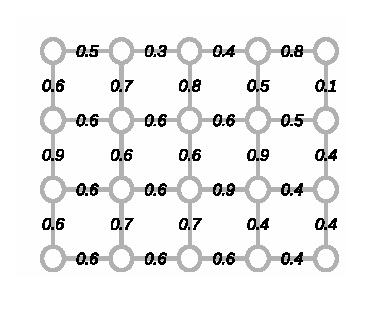
\includegraphics[scale=0.66]{fig/affinity_graph}}
  \subfloat[]{\protect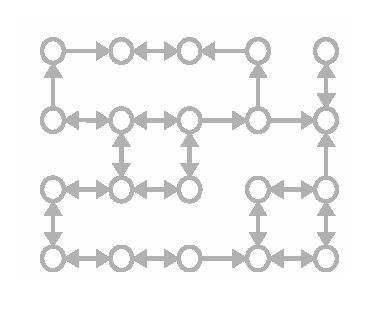
\includegraphics[scale=0.66]{fig/sd_graph}}\\
  \subfloat[]{\protect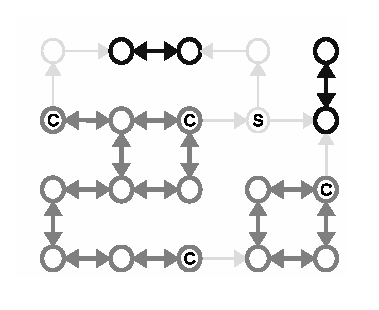
\includegraphics[scale=0.66]{fig/sd_graph_plateaus}}
  \subfloat[]{\protect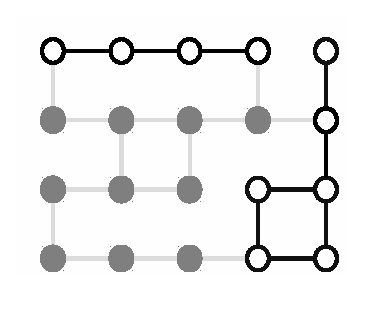
\includegraphics[scale=0.66]{fig/ws_result}}

  \protect\caption{The plateau division problem. (a) Affinity graph;
    (b) Retaining only maximal edges for each vertex yields this
    steepest ascent graph; (c) locally maximal plateaus (black),
    non-maximal plateau (dark gray), saddle vertex (S), plateau
    corners (C); (d) the two basins of attractions and border vertices
    (dark gray)}
\end{figure}

\subsection{Steepest ascent graph}
The inputs to the algorithm are an undirected weighted graph $G$, and
an ordering of the vertices of $G$ that is used for tie-breaking. The
ordering could be represented by a bijective map
$\alpha:V\to\{1,2,...,|V|\}$. We refer to $\alpha(u)$ as the index of
$u$ (Fig. 2a).

Replace each edge of $G$ by edges in both directions between the same
vertices (Fig. 1(a)).  Then for every vertex retain the outgoing edge
with maximal weight and eliminate other outgoing edges.  The resulting
graph, called $D_1$ is directed and unweighted.  If there are ties
between outgoing edges (Fig. 1b), they are resolved by using the
vertex ordering.  The winning edge is the one pointing to the vertex
with the lowest index.

By construction, any directed path in $D_1$ is a path of steepest
ascent in $G$.  If a pair of vertices has edges in both directions,
they are represented by a single ``bidirectional edge'' in Fig. 1b.
Therefore, the edges of any vertex in $D_1$ can be classified as
incoming, outgoing, and bidirectional.

%A steepest descent graph can be defined analogously using edges of minimal weight. Either steepest ascent or descent can be used without loss of generality.

\begin{figure}
  \centering
  \subfloat[]{\protect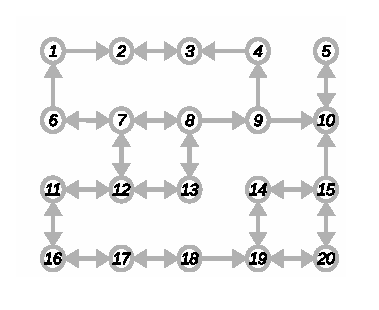
\includegraphics[scale=0.66]{fig/sd_graph_ordered}}
  \subfloat[]{\protect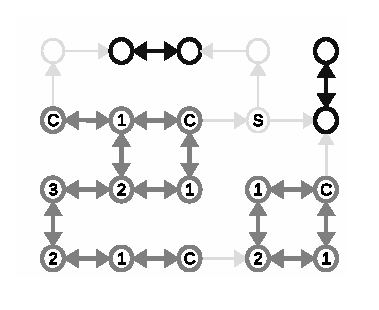
\includegraphics[scale=0.66]{fig/sd_graph_plateaus_ordered}}\\
  \subfloat[]{\protect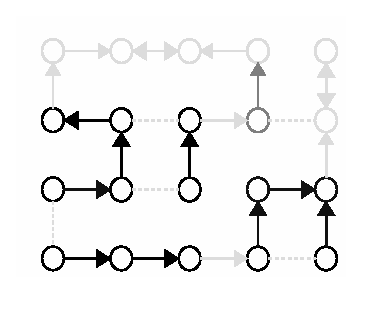
\includegraphics[scale=0.66]{fig/sd_graph_plateaus_modified}}
  \subfloat[]{\protect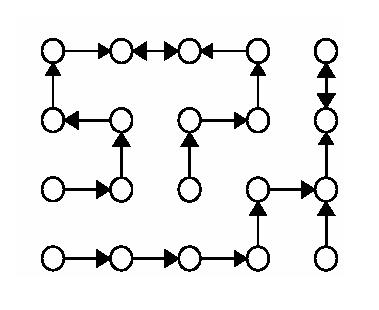
\includegraphics[scale=0.66]{fig/final_segmentation}}

  \protect\caption{Watershed algorithm that divides plateaus
    evenly. (a) existence of a vertex ordering is assumed; (b) Every
    plateau vertex is labeled by its graph distance to the nearest
    plateau corner; (c) the steepest ascent graph defines unique paths;
    (d) final watershed segmentation}
\end{figure}

\subsection{Plateau division}
Directed paths in $D_1$ may not be unique, if plateaus exist.  A
\emph{plateau} is a connected component of the subgraph of $D_1$
containing only bidirectional edges.  A plateau \emph{corner} is a
plateau vertex with an outgoing edge.
% there can't be more than one, since saddles were eliminated, right?
\emph{Locally maximal} plateaus contain no corners; they are
equivalent to the regional maxima of the original graph.  If a
directed path of $D_1$ enters a locally maximal plateau, it remains
within the plateau for all future time.

\emph{Non-maximal} plateaus contain one or more corners.  If a
directed path enters a non-maximal plateau, it may stay within the
plateau, or exit through one of the corners.  These types
of plateaus are illustrated in Fig. 1c.

We would like to alter $D_1$ so that any directed path that enters a
non-maximal plateau will not get stuck there, but will eventually
exit.  This guarantees that any directed path will eventually reach a
regional maximum, i.e., regional maxima are attractors of the dynamics.

Furthermore, we would like a non-maximal plateau with multiple corners
to be divided evenly, in the following sense.  From each vertex in the
plateau, the directed path should lead to the nearest corner, where
nearest is defined based on graph distance.  If there is a tie between
corners, it should be resolved using the same vertex ordering as
before.  Both of these goals are achieved for a non-maximal plateau by
performing a breadth first search (BFS) for all of its vertices,
starting from its corners with the vertex ordering.

The BFS proceeds as follows.  We initialize a global FIFO queue $Q$,
mark all the corner vertices as visited and insert them into $Q$ in
increasing order of their index. While $Q$ is not empty we remove the
vertex $v$ from the front of the queue, and loop over all its
bidirectional edges $\{v,u\}$.  If $u$ has not yet been visited, we
mark it as visited, insert it to the back of the queue, and change the
edge from bidirectional to incoming $(v\leftarrow u)$. If $u$ has
already been visited, we remove the bidirectional edge $\{v,u\}$
completely.

\subsection{Connected components}
After applying this BFS to every non-maximal plateau, we arrive at the
modified steepest ascent graph $D_2$ (Fig. 2c).  Every directed path eventually reaches a locally maximal plateau.  The path from any vertex to its corresponding regional maximum is unique.  Therefore, the graph can be segmented into the basins of attraction of the dynamics.

The basins can be found by regarding $D_2$ as an undirected graph and
computing its connected components.  [via what algorithm]

\subsection{Time complexity}
As we operate on a connected graph we assume $O(|E|) \ge O(|V|)$.  To
create $D_1$, we visit each edge a constant number of times. To create
$D_2$, we visit each vertex at most once, and edges incident to it a
constant number of times. The complexity of connected components is
$O(|E|)$.  Therefore the overall complexity is $O(|E|)$.

\subsection{Properties of watershed segmentation}
The algorithm produces an optimal partitioning as defined
in~\cite{Cousty2009}.

Basins are in one-to-one correspondence with regional maxima.

maximal spanning forest
steepest ascent graph in each basin is maximal spanning tree?

\section{Hierarchical watershed segmentation}
Many methods have been proposed for turning a flat watershed
segmentation into a hierarchical segmentation.  Most methods amount to
some kind of agglomerative clustering algorithm applied to the
watershed basins \cite{beucher1994watershed, Najman1996}.  Here we
propose the use of single linkage clustering.  Although this is a
relatively simple and perhaps even naive method, it is worth
considering because it is (1) efficiently computable and (2) leads to
a definition of hierarchy that is particularly ``natural,'' in a way
that will be made precise below.

\subsection{Single linkage clustering}
In single linkage clustering, the affinity of two clusters is defined
as the maximal affinity of all edges between the two clusters.  At
each step, a pair of clusters with maximum affinity is merged.  The
output is a dendrogram.  The height of each branch point is given by
the affinity at which the two clusters merge.

[describe efficient algorithm and its time complexity]

% maximin affinity between two regional maxima in two clusters

\begin{figure}
\caption{dendrogram goes here}
\end{figure}

\subsection{Upper thresholding of the affinity graph}
Above we claimed that single linkage clustering leads to a definition
of hierarchy that is particularly ``natural'' for watershed.  The
rationale for this claim is as follows.  Suppose that the original
affinity graph were modified by replacing all affinities larger than
$\theta_{\max}$ by a common high value (e.g. $\infty$).  The flat watershed
segmentation of the modified affinity graph would correspond to one of
the levels of the hierarchical segmentation produced by single linkage
clustering.

To prove this, we first prove the following lemma:
\begin{lemma}
  Let $G'$ be the affinity graph obtained by setting all affinities of
  $G$ greater than $\theta$ to a common high value (e.g. $\infty$).
  Let $W=\{B_1,B_2,\dots\}$ and $W'=\{B'_1,B'_2,\dots\}$ be the
  watershed segmentations of $G$ and $G'$, respectively.  For each
  $B_i$ there exists $B'_j$ such that $B_i \subseteq B'_j$.
\end{lemma}

\begin{proof}
Let $S_2$ and $S_2'$ be the steepest ascent graphs obtained from $G$
and $G'$, respectively.  Vertices of $S_2$ not incident to any edge
with affinity smaller than $\theta$ will stay unmodified, even after
plateau division. All other vertices of $S_2$ will become part of a
locally maximal plateau of $S_2'$ (regional maximum of $G'$). All
locally maximal edges of $S_2$ will stay locally maximal. Therefore
the only effect of the affinity threshold is to introduce
bidirectional edges. Therefore, a connected component of $S_2$ has to
be a subset of a connected component of $S_2'$
\end{proof}

Now we are ready to prove the following theorem.
\begin{theorem}
The following are equivalent:
\begin{enumerate}
\item Watershed segmentation of $G$ followed by single linkage clustering of basins down to affinity $\theta$.
\item Creation of $G'$ from $G$ by replacing all affinities larger
  than $\theta$ by a common high value (e.g. $\infty$), followed by
  watershed segmentation of $G'$.
\end{enumerate}
\end{theorem}

\begin{proof}
Watershed basins are connected. By the Lemma, each $W'$ basin is the
union of one or more $W$ basins. We will prove that two $W$ basins are
merged by single linkage clustering down to affinity $\theta$ if and
only if they belong to the same $W'$ basin.

Suppose that $B_i$ and $B_j$ are merged by single linkage clustering
down to affinity $\theta_{\max}$.  This means that there exists an
edge in $G$ connecting the two basins with affinity larger than
$\theta$. The edge and its two vertices will belong to some regional
maximum of $G'$, and hence a single basin of $W'$.  It follows the two
basins of $W$ belong to a single basin of $W'$.

Conversely, suppose that $B_i$ and $B_j$ belong to the same $W'$
basin.  Then there exists a steepest ascent path

$\theta_{\max}$, then there exists an edge $\{u,v\}$ in $G$ such that
$u \in B_i$ and $v \in B_j$ with the weight equal to $d_{ij} <
T_{\min}$. Therefore $u$ and $v$ will be part of the same regional
minima, and $B_i$ and $B_j$ will be part of the same watershed basin
in $W'$.
\end{proof}

\section{Source code}
3D image
Nearest neighbor affinity graph 

\section{Discussion}
To show confidence about high values of \emph{disaffinities}, and in
order to prevent undesired mergers, we introduce a threshold
$\theta_{\min}$ by eliminating all edges with affinity less than
$\theta_{\min}$. The lower threshold can produce singleton vertices in
$G$. The singleton vertices are not assigned to any watershed basin
and are considered background, which is often a desired result.

mention possible improvements to hierarchy

Like watershed cuts, our algorithm has linear time complexity.  The
use of multiple passes makes it possible to divide plateaus evenly.  A
second motivation for our algorithm is that it separates the
computation into two passes that are parallelizable versus two passes
that are not.  A parallel variant of our algorithm will be described
in a future paper.



%%%%%%%%%%%%%%%%%%%%%%%%%%%%%%%%%%%%%%%%%%%%%%%%%%%%%%%%%%%%%%%%%%%%%%%
%%%%%%%%%%%%%%%%%%%%%%%%%%%%%%%%%%%%%%%%%%%%%%%%%%%%%%%%%%%%%%%%%%%%%%%
%%
%% REFERENCES
%%
%%%%%%%%%%%%%%%%%%%%%%%%%%%%%%%%%%%%%%%%%%%%%%%%%%%%%%%%%%%%%%%%%%%%%%%
%%%%%%%%%%%%%%%%%%%%%%%%%%%%%%%%%%%%%%%%%%%%%%%%%%%%%%%%%%%%%%%%%%%%%%%


{\small
\bibliographystyle{ieeetr}
\bibliography{./ref/bib}
}

\end{document}

\subsection{Assigning border vertices}
In Fig. 1(d) we show the \emph{basins of attraction} of the two
\emph{regional minima}. The \emph{border} vertices are shown in dark
gray and belong to both \emph{basins of attraction}. Watershed
cuts~\cite{Cousty2009,Cousty2010} assign \emph{border} vertices with a
single constraint that all the \emph{basins of attraction} have to be
connected.

